%!TEX root = ../dissertation.tex
\chapter{Analisi e progettazione}
In questo capitolo analizzeremo le metodologie di lavoro, i problemi riscontrati e i risultati ottenuti.
\section{Metodo di lavoro}
Dopo un'attenta analisi delle esigenze di questo progetto, la metodologia che abbiamo deciso di utilizzare è Agile Kanban. Questa metodologia, ci ha permesso di avere un'alta flessibilità sui task da svolgere, una visione ampia del progetto e il focus su una singola attività alla volta.
La metodologia Kanban è stata scelta anche per affrontare l'esiguo numero del team, composto da sole 2 persone, con effettivamente solo una che lavorava a pieno regime su di esso.
Questo perché rendeva un'ottima visione dell'insieme delle attività da svolgere, in progresso e già svolte, oltre a non necessitare di ruoli predefiniti come nell'\gls{Agile Scrum}
\paragraph{Metodologia kanban}
Fa parte della famiglia delle metodologie agile, alla base vi è l'utilizzo di una lavagna nella quale vi è specificato uno stato per ogni colonna presente.
\begin{figure}[h!]
	\centering
	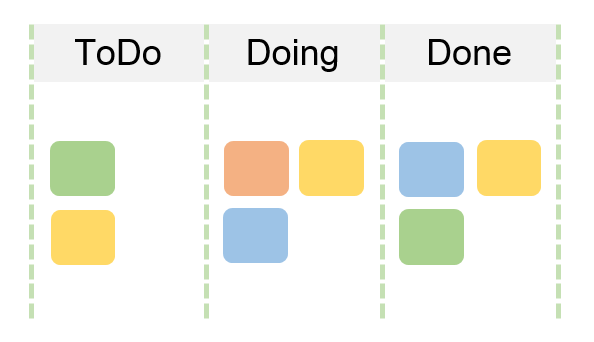
\includegraphics[scale=0.3]{figures/kanban-board}
	\caption[Esempio lavagna Kanban.]{Esempio lavagna Kanban.
		\label{fig:logoGCP}}
\end{figure}	
Quello sopra riportato è uno degli esempi più semplici di lavagna Kanban, nella quale ogni task deve assumere tre stati per considerarsi completato "ToDo", "Doing" e "Done". Solitamente ogni componente del team ha la responsabilità di portare a completamente un solo task alla volta, così da evitare sovrapposizioni e confusione.
\\ 
Questa metodologia ha sicuramente giovato al progetto dato l'alto livello di flessibilità garantito e necessario al rispetto dalle richieste periodiche del cliente.
\paragraph{Trello}
Dato che i componenti del team difficilmente sarebbero riusciti a condividere lo stesso spazio di lavoro, inteso come luogo fisico, abbiamo deciso di utilizzare una lavagna digitale fornita da Trello.
\\ Trello rende disponibile gratuitamente online un ottima implementazione dei principi esposti all'interno della metodologia Kanban, gli elementi chiave risultano essere 3: la lavagna, le liste (o anche colonne della lavagna) e le card (cioè i singoli task).
\begin{figure}[h!]
	\centering
	
\includegraphics[scale=0.08]{figures/trello-logo}
	\caption[Logo Trello]{Logo di Trello \cite{trello}.
		\label{fig:logoGCP}}
\end{figure}
\section{Problemi affrontati}
Affrontare sfide, problemi e quesiti di carattere tecnologico, architetturale e implementativo è stata sicuramente la parte più formativa del periodo di stage, dato che in queste situazioni lo studio autonomo e il confronto con esperti del settore come il mio Tutor sono stati di primaria importanza.
\\
I problemi affrontati durante questo progetto sono molteplici e vanno dall'analisi e scelta delle tecnologie da utilizzare all'integrazione tra le stesse.
\\
Per circoscrivere le problematiche abbiamo deciso di sviluppare il progetto in due sotto-progetti autonomi. 
Il primo tratta dell'ingestion dei dati e il secondo dell'utilizzo dei dati con il fine di categorizzare gli utenti. Da questi quindi, derivano diverse tipologie di problemi, tra cui la scelta e lo studio degli strumenti e delle \gls{best practices}.
\\
Il punto cruciale del sotto-progetto riguardante l'ingestion è stato lo studio delle tecnologie riguardanti Google Cloud Platform e con esso le conseguenti scelte obbligate, come lo studio di Apache Beam, l'utilizzo di sole librerie compatibili con Google Cloud ed i suoi strumenti.
\\
Per quanto riguarda la classificazione degli utenti, si è scelto di intraprendere una strada che potesse portare a dei vantaggi di utilizzo e portabilità, cioè si è deciso di utilizzare un \gls{container} Docker per lo sviluppo ed utilizzo degli algoritmi di classificazione.
Questo è stato fatto per agevolare l'installazione e configurazione in locale dell'intero pacchetto di strumenti da utilizzare, tra cui Spark, Kafka e Hadoop.
Ovviamente, l'utilizzo di Docker ha comportato la scelta del miglior compromesso per la creazione di un container adatto. Dato l'ampio pacchetto di strumenti da studiare in autonomia, abbiamo deciso quindi di utilizzare un container Cloudera \cite{containercloudera} già contenete la maggior parte degli strumenti necessari per sviluppare un processo di classificazione degli utenti.
Inoltre, per far si che i dati venissero continuamente aggiornati, come effettivamente succede nella fase di ingestion, abbiamo deciso di utilizzare Kafka Straming per mantenere un flusso continuo di verifica delle anomalie, così da mantenere in costante aggiornamento il cliente.

\section{Requisiti}
\subsection{Struttura}
Ogni requisito è descritto dalla seguente struttura:
\begin{itemize}
	\item Tipo;
	\item Importanza;
	\item Stato implementazione;
	\item Fonti.
\end{itemize}

Inoltre, a ciascun requisito corrisponde un codice identificativo cosi composto:
$$ \textbf{R \{importanza\}.\{tipo\}.\{identificativo\}  } $$
\begin{itemize}
	\item R specifica che si tratta di un requisito;
	\item importanza identifica la rilevanza del requisito e può assumere 3 valori:
	\begin{itemize}
		\item 0: indica che il requisito è obbligatorio e il suo soddisfacimento dovrà necessariamente avvenire;
		\item 1: indica che il requisito è desiderabile, cioè il suo soddisfacimento può portare maggiore completezza al sistema ma non è fondamentale per lo stesso;
		\item 2: indica che il requisito è opzionale, e quindi la decisione di implementarlo o meno verrà presa dopo le dovute considerazioni.
	\end{itemize}
	\item tipo distingue se si tratta di un requisito funzionale (F), di qualità (Q), di prestazione (P) o di vincolo (V);
	\item identificativo è un numero progressivo che identifica i sottocasi.
\end{itemize}
	\newcolumntype{H}{>{\centering\arraybackslash}m{9.5cm}}
\subsection{Tabella dei requisiti}
Per assolvere gli obiettivi del progetto e per rispondere in modo concreto ai problemi sorti, durante lo stage sono stati definiti i seguenti requisiti.
\normalsize
\renewcommand{\arraystretch}{1.5}
\begin{longtable}{|c|H|c|}
	\hline
	\textbf{Id Requisito} &
	\textbf{Descrizione} &
	\textbf{Fonte}\\
	\hline
	\endhead
	\hypertarget{R0F1}{R0F1} & Il sistema deve essere in grado di trasferire i file con estensione evtx e xml dal server SFTP a Google Cloud Storage. & Interno  \\ \hline 	 
	\hypertarget{R1F1.1}{R1F1.1} & Il sistema deve essere in grado di verificare la corretta estensione dei file. & Interno  \\ \hline 	 
	\hypertarget{R1F1.2}{R1F1.2} & Il sistema deve essere in grado di scartare i file con una non corretta estensione. & Interno  \\ \hline 	 
	\hypertarget{R1F1.3}{R1F1.3} & Il sistema deve essere in grado di validare i file con estensione evtx. & Interno  \\ \hline 	 
	\hypertarget{R1F1.4}{R1F1.4} & Il sistema deve essere in grado di convertire i file evtx in xml. & Interno  \\ \hline 	 
	\hypertarget{R0F2}{R0F2} & Il sistema deve essere in gardo di aggiornarsi periodicamente. & Interno  \\ \hline 	 
	\hypertarget{R1F2.1}{R1F2.1} & Il sistema deve essere in gardo verificare la presenza di nuovi file all'interno del server SFTP. & Interno  \\ \hline 	 
	\hypertarget{R1F2.2}{R1F2.2} & Il sistema deve essere in gardo di avviare il processo di ingestion dei file ad ogni nuovo arrivo. & Interno  \\ \hline 	 
	\hypertarget{R1F2.2.1}{R1F2.2.1} & Il sistema deve essere in gardo di notificare l'arrivo di nuovi file all'interno del Bucket Google Cloud Storage. & Interno  \\ \hline 	 
	\hypertarget{R1F2.2.2}{R1F2.2.2} & Il sistema deve essere in gardo di avviare il processo di ingestion una volta ricevuta la notifica dal Bucket Google Cloud Storage. & Interno  \\ \hline 	 
	\hypertarget{R0F3}{R0F3} & Il sistema deve essere in grado di processare i flussi batch producendo i dataset di output
	richiesti. & Interno  \\ \hline 	 
	\hypertarget{R0F3.1}{R0F3.1} & Il sistema deve essere in gardo di archiviare i file di output all'interno del Bucket Google Cloud Storage. & Interno  \\ \hline 	 
	\hypertarget{R1F3.2}{R1F3.2} & Il sistema deve essere in gardo di archiviare i file di output all'interno di Google Cloud BigQuery. & Interno  \\ \hline 	 
	\hypertarget{R0F4}{R0F4} & I processi devono essere schedulati per avviarsi periodicamente. & Interno  \\ \hline 	 
	\hypertarget{R1F5}{R1F5} & Il sistema deve riuscire ad aggiornarsi continuamente senza interrompere l’erogazione del
	servizio. & Interno  \\ \hline 	 
	\hypertarget{R1F6}{R1F6} & Il sistema deve essere in grado di scrivere i risultati su una struttura interrogabile via SQL. & Interno  \\ \hline 	 

	\hypertarget{R1F7}{R1F7} & Il sistema deve essere in grado di classificare i dati all'interno dei file provenienti dal processo di ingestion. & Interno  \\ \hline 	 
	\hypertarget{R1F7.1}{R1F7.1} & Il sistema deve essere in grado di classificare i dati all'interno dei file provenienti dal processo di ingestion per singolo giorno. & Interno  \\ \hline
	\hypertarget{R1F7.2}{R1F7.2} & Il sistema deve essere in grado di classificare i dati all'interno dei file provenienti dal processo di ingestion per singolo file su base multi-giorno. & Interno  \\ \hline 	 
	\hypertarget{R1F8}{R1F8} & Il sistema deve essere in grado di inviare una email al manager responsabile in caso di anomalie nei dati classificati. & Interno  \\ \hline 	 

	\hypertarget{R1F9}{R1F9} & Il sistema deve essere in grado di rendere visibile dei report all'interno di Google Data Studio. & Interno  \\ \hline 	 
	\hypertarget{R2F10}{R2F10} & Il sistema deve poter lavorare su dati archiviati su Elasticsearch. & Interno  \\ \hline 	 
	\hypertarget{R2F11}{R2F11} & Il sistema deve poter essere in grado di scrivere i propri output su DB NoSQL. & Interno  \\ \hline 	 
	\hypertarget{R0Q1}{R0Q1} & La progettazione e il codice devono
	seguire le norme riportate all'interno degli standard di Data Reply S.r.l. & Interno  \\ \hline 	 
	\hypertarget{R0Q2}{R0Q2} & Tutti i documenti e il codice prodotto
	devono rispettare le metriche riportate all'interno degli standard di Data Reply S.r.l. & Interno  \\ \hline 	 
	\hypertarget{R0Q3}{R0Q3} & Deve essere prodotto un manuale
	sviluppatore. & Interno  \\ \hline 	 
	\hypertarget{R0V1}{R0V1} & Il sistema deve utilizzare strumenti appartenenti a Google Cloud Platform o ad esso compatibili. & Interno  \\ \hline 	 
	\hypertarget{R1V1}{R1V1} & Il sistema deve utilizzare Spark MLlib per il sistema di classificazione. & Interno  \\ \hline 	 
	\hypertarget{R2V1}{R2V1} & Il sistema di classificazione deve essere sviluppato all'interno di un container Docker. & Interno  \\ \hline 	 
	\hypertarget{R1P1}{R1P1} & Il sistema deve poter scalare le risorse in base al volume di dati. & Interno  \\ \hline 	 
	\caption[Requisiti Di Vincolo]{Requisiti di Vincolo}
	\label{tabella:req3}
\end{longtable}
\renewcommand{\arraystretch}{1}


\section{Pianificazione del lavoro}
Durante i colloqui svolti con il tutor aziendale, è stato redatto il piano di lavoro. Ciò ha portato la suddivisione dello stage in 8 parti, ognuna della durata di una settimana.
    \begin{itemize}
	\item[] \textbf{Prima Settimana (40 ore)}
	\begin{itemize}
		\item Incontro con persone coinvolte nel progetto per discutere i requisiti e le richieste
		relativamente al sistema da sviluppare;
		\item Verifica credenziali e strumenti di lavoro assegnati;
		\item Presa visione dell’infrastruttura esistente;
		\item Formazione sulle tecnologie adottate.
	\end{itemize}
	\item[] \textbf{Seconda Settimana (40 ore)} 
	\begin{itemize}
		\item Comprensione strumenti di storicizzazione;
		\item Analisi funzionamento filesystem distribuito;
		\item Produzione script Python per produzione dati simulati.
	\end{itemize}
	\item[] \textbf{Terza Settimana (40 ore)} 
	\begin{itemize}
		\item Caricamento dati su filesystem distribuito;
		\item Securizzazione accesso ai dati;
		\item Studio teorico approccio statistico al problema.
	\end{itemize}
	\item[] \textbf{Quarta Settimana (40 ore)} 
	\begin{itemize}
		\item Comprensione strumenti di processamento;
		\item Analisi funzionamento RDD;
		\item Implementazione processo batch con Python e Spark.        
	\end{itemize}
	\item[] \textbf{Quinta Settimana (40 ore)} 
	\begin{itemize}
		\item Analisi funzionamento Dataframe;
		\item Implementazione processo di elaborazione Spark;
		\item Ingegnerizzazione soluzione batch.
	\end{itemize}
	\item[] \textbf{Sesta Settimana (40 ore)} 
	\begin{itemize}
		\item Test prestazionale processo spark;
		\item Tuning prestazionale;
		\item Studio applicazione real-time.
	\end{itemize}
	\item[] \textbf{Settima Settimana (40 ore)} 
	\begin{itemize}
		\item Storicizzazione dati su storage persistente;
		\item Studio funzionamento Kafka;
		\item Implementazione processo real-time con Spark Streaming.
	\end{itemize}
	\item[] \textbf{Ottava Settimana - Conclusione (40 ore)} 
	\begin{itemize}
		\item Costruzione layer accesso al dato persistente;
		\item Ingegnerizzazione soluzione Spark Streaming;
		\item Integrazione storage persistente.
	\end{itemize}
\end{itemize}
possibili diagrammi.
\section{Risultati}
Alla fine del periodo di stage, i risultati ottenuti sono stati considerati più che positivi dal tutor aziendale Dott. Michele Giusto, dato che sono stati soddisfatti tutti i requisiti obbligatori e desiderabili. I requisiti facoltativi, non sono stati implementati per lasciare maggiore spazio e importanza ai requisiti obbligatori.
\\
Inoltre, il sotto-progetto riguardante la fase di ingestion ha avuto ottimi risultati, tale per cui si è dimostrata pronta per essere utilizzata in fasi di "produzione".
Per quanto riguarda la parte di classificazione, è stata messa a punto per scheletro e funzionalità senza però essere pronta per gestire effettivamente l'aggiornamento real time dei dati, soprattutto perché da parte del clienti vi è stato un rallentamento nel passaggio di dati ed informazioni per la scelta del miglior modello. 


